\documentclass[german,10pt]{book}      
\usepackage{makeidx}
\usepackage{babel}            % Sprachunterstuetzung
\usepackage{amsmath}          % AMS "Grundpaket"
\usepackage{amssymb,amsfonts,amsthm,amscd} 
\usepackage{mathrsfs}
\usepackage{rotating}
\usepackage{sidecap}
\usepackage{graphicx}
\usepackage{color}
\usepackage{fancybox}
\usepackage{tikz}
\usetikzlibrary{arrows,snakes,backgrounds}
\usepackage{hyperref}
\hypersetup{colorlinks=true,
                    linkcolor=blue,
                    filecolor=magenta,
                    urlcolor=cyan,
                    pdftitle={Overleaf Example},
                    pdfpagemode=FullScreen,}
%\newcommand{\hyperref}[1]{\ref{#1}}
%
\definecolor{Gray}{gray}{0.80}
\DeclareMathSymbol{,}{\mathord}{letters}{"3B}
%
\newcounter{num}
\renewcommand{\thenum}{\arabic{num}}
\newenvironment{anmerkungen}
   {\begin{list}{(\thenum)}{%
   \usecounter{num}%
   \leftmargin0pt
   \itemindent5pt
   \topsep0pt
   \labelwidth0pt}%
   }{\end{list}}
%
\renewcommand{\arraystretch}{1.15}                % in Formeln und Tabellen   
\renewcommand{\baselinestretch}{1.15}                 % 1.15 facher
                                                      % Zeilenabst.
\newcommand{\Anmerkung}[1]{{\begin{footnotesize}#1 \end{footnotesize}}\\[0.2cm]}
\newcommand{\comment}[1]{}
\setlength{\parindent}{0em}           % Nicht einruecken am Anfang der Zeile 

\setlength{\textwidth}{15.4cm}
\setlength{\textheight}{23.0cm}
\setlength{\oddsidemargin}{1.0mm} 
\setlength{\evensidemargin}{-6.5mm}
\setlength{\topmargin}{-10mm} 
\setlength{\headheight}{0mm}
\newcommand{\identity}{{\bf 1}}
%
\newcommand{\vs}{\vspace{0.3cm}}
\newcommand{\noi}{\noindent}
\newcommand{\leer}{}

\newcommand{\engl}[1]{[\textit{#1}]}
\parindent 1.2cm
\sloppy

         \begin{document}  %\setcounter{chapter}{7}

%\newcommand{\solution}[1]{}

\chapter{Zustands- und Prozessgr\"o\ss en}
% Kap x
\label{chap_Zustand}

Der erste Hauptsatz der Thermodynamik -- die Erhaltung der Energie -- wird
in\index{Thermodynamik!erster Hauptsatz}\index{Erster Hauptsatz der Thermodynamik}\index{Energieerhaltung} 
der Thermodynamik gerne in folgender Form zum Ausdruck gebracht:
\begin{equation}
\label{eq_ZuPro_Energie}
                {\rm d} U = \delta Q - \delta W \, .
\end{equation}
Physikalisch bedeuten ${\rm d}U$ eine \glqq infinitesimale\grqq\ \"Anderung
der inneren Energie eines Systems, $\delta Q$ die dem System zugeflossene
W\"arme und $\delta W$ die vom System an der Umgebung geleistete 
Arbeit.\index{Waerme@W\"arme}\index{Arbeit}\index{Innere Energie}
Die Gleichung besagt somit, dass eine \"Anderung der inneren Energie eines Systems
nur durch einen Fluss an Energie in oder aus dem System erfolgen kann -- in diesem
Sinne handelt es sich um eine Kontinuit\"atsgleichung f\"ur die Energie; Energie kann
innerhalb eines Systems weder erzeugt noch vernichtet werden -- und dass
dieser Energiefluss auf zwei Weisen erfolgen kann: als W\"arme oder in Form von
Arbeit, die makroskopisch kontrolliert werden kann. 

Diese Formulierung des ersten Hauptsatzes wirft zwei Fragen auf:
\begin{enumerate}
\item
Weshalb verwendet man das Symbol ${\rm d}$ bei der inneren Energie U
und das Symbol $\delta$ bei der W\"arme und der Arbeit (manchmal findet man auch
das Symbol ${\rm \dj}$ oder andere Bezeichnungen)? Worin besteht
der Unterschied bzw.\ was soll damit zum Ausdruck gebracht werden? 
\item
Wie kann man den W\"armefluss von dem Fluss an Arbeit unterscheiden, bzw.\
wie sind diese beiden Gr\"o\ss en genau definiert?
\end{enumerate}

Die Beantwortung der ersten Frage wird uns in Abschnitt \ref{sec_ZuPro} zun\"achst auf den Unterschied 
zwischen Zustands- und Prozessgr\"o\ss en f\"uhren und wir werden erl\"autern, weshalb es sich 
bei Gl.\ \ref{eq_ZuPro_Energie} um eine Gleichung zwischen Prozessgr\"o\ss en handelt. 
Diese Prozessgr\"o\ss en (mathematisch handelt es sich um 1-Formen) 
k\"onnen das Differential einer Zustandsgr\"o\ss e sein, d.h.\ einer Funktion auf dem Raum der 
Gleichgewichtszust\"ande (in diesem Fall verwenden wir das Symbol ${\rm d}$), oder auch Felder, die sich nicht
als Gradient bzw.\ Differential einer Zustandsgr\"o\ss e ausdr\"ucken lassen und die man an einem 
Gleichgewichtszustand nicht messen kann (in diesem Fall verwenden wir das Symbol $\delta$). 
Mathematisch orientierte Lehrb\"ucher bzw.\
Texte (z.B.\ \cite{Jauch,Straumann}) legen Wert darauf, dass es sich hierbei nicht
um \glqq infinitesimale\grqq\ Gr\"o\ss en handelt, sondern um lineare Abbildungen (Formen), 
die endliche Werte annehmen (und sie vermeiden daher die Symbole d und $\delta$). 
Das f\"uhrt auf die Frage, weshalb das anschauliche Bild von
\glqq kleinen Gr\"o\ss en\grqq\ trotzdem nicht falsch zu sein scheint und wie sich dieses
Bild mit der mathematischen Vorstellung von 1-Formen vertr\"agt. 

\section{Die Mannigfaltigkeit der Gleichgewichtszust\"ande}

Die Thermodynamik besch\"aftigt sich mit sogenannten 
Gleichgewichtszust\"anden\index{Gleichgewichtszustand}
sowie den \"Uberg\"angen zwischen Gleichgewichtszust\"anden. Dabei ist ein \textit{Gleichgewichtszustand}
ein Zustand, der sich bei einem System nach ausreichend langer Zeit einstellt und bei
dem sich makroskopisch beobachtbare Kenngr\"o\ss en des Systems (Volumen, Druck,
Temperatur, Stoffmengen, etc.) nicht mehr \"andern. Das setzt voraus, dass das
System entweder vollkommen abgeschlossen ist oder aber in Kontakt mit einer Umgebung
steht, die selbst keinen Ver\"anderungen unterliegt. Solche Gleichgewichtszust\"ande lassen
sich meist durch wenige (endlich viele) Kenngr\"o\ss en charakterisieren, wobei diese
Kenngr\"o\ss en nicht unabh\"angig voneinander sind, sondern durch sogenannte
\textit{Zustandsgleichungen} verkn\"upft sind.\index{Zustandsgleichung}
Man kann nun einen maximalen Satz von
unabh\"angigen Kenngr\"o\ss en zur Charakterisierung der Zust\"ande heranziehen, 
z.B.\ Druck, Volumen und Stoffmenge bei einem idealen Gas. Diese bezeichnet man auch
manchmal als \textit{Arbeitskoordinaten}.\index{Arbeitskoordinaten}  
Die Temperatur ist dann\index{Temperatur}
eine abh\"angige Kenngr\"o\ss e, die \"uber die thermische Zustandsgleichung (z.B.\ die
ideale Gasgleichung\index{Gasgleichung, ideale}\index{Ideales Gas}\index{Thermische Zustandsgleichung}
$pV=nRT$; $p$ Druck, $V$ Volumen, $n$ Stoffmenge in Mol, $R$ Gaskonstante und $T$
Temperatur) mit den unabh\"angigen Gr\"o\ss en verkn\"upft ist. Auch die Energie eines
idealen Gases l\"asst sich durch diese Gr\"o\ss en ausdr\"ucken: $E=\frac{3}{2}pV$. 

F\"ur manche formalen \"Uberlegungen (z.B.\ zu Gl.\ \ref{eq_ZuPro_Energie}) ist es sinnvoll, die
Energie zu den unabh\"angigen Kenngr\"o\ss en zu z\"ahlen, 
ebenso wie das Volumen und die Stoffmenge (entweder ausgedr\"uckt durch\index{Stoffmenge}
die Teilchenzahlen $N_i$ bei verschiedenen durch $i$ nummerierten Stoffarten oder
aber ausgedr\"uckt durch die Molzahl $n_i = N_i/N_{\rm A}$, wobei $N_{\rm A}=6,022\,140\,76 \cdot
10^{23}$ die Avogadro-Zahl ist)\index{Avogadro-Zahl}\index{Molzahl} 
sowie andere Gr\"o\ss en, mit denen wir die von dem System
(in welcher Form auch immer) geleistete Arbeit kontrollieren (mehr dazu in Abschnitt \ref{sec_ZuPro_Arbeit}).
Bei einem mechanischen System w\"are die Energie dann eine abh\"angige Gr\"o\ss e, doch da
in der Thermodynamik noch die Zustandsgr\"o\ss e Temperatur hinzukommt (die man nicht zu
den Arbeitskoordinaten z\"ahlen w\"urde), wird die Energie zu einer unabh\"angigen Gr\"o\ss e. 

Wir stellen uns nun die Menge aller Gleichgewichtszust\"ande als eine Mannigfaltigkeit $M$
vor.\index{Mannigfaltigkeit!der Gleichgewichtszust\"ande} 
Das bedeutet, wir k\"onnen Gleichgewichtszust\"ande $p\in M$ durch Koordinaten 
$p\simeq (x_1(p),...,x_n(p))$ charakterisieren ($x_i$ sind die oben erw\"ahnten Arbeitskoordinaten 
bzw.\ unabh\"angigen Kenngr\"o\ss en) und wir k\"onnen diese
Koordinaten \"uber bestimmte Bereiche hinweg stetig variieren und beschreiben damit sinnvolle
und ebenfalls stetig verbundene Gleichgewichtszust\"ande eines Systems.\footnote{Wie immer
in der Physik verlangen wir auch die f\"ur alle Operationen notwendigen Ableitbarkeitsbedingungen.
Das ist gelegentlich bei Phasen\"uberg\"angen nicht der Fall.}    

Unter einem \textit{quasistation\"aren Prozess}\index{Prozess}\index{Prozess!quasistation\"ar} 
versteht man einen Weg auf der Mannigfaltigkeit\index{Quasistation\"arer Prozess}
der Gleichgewichtszust\"ande, d.h.\ eine Abbildung $\gamma: [0,1] \longrightarrow M$, meist
ausgedr\"uckt durch die Koordinaten $\gamma: t \mapsto \pmb{x}(t) = (x_1(t),...,x_n(t))$.
Der Parameter $t$ muss nicht unbedingt die Zeit bedeuten. Damit sich ein solcher Prozess 
tats\"achlich auf der Mannigfaltigkeit der Gleichgewichtszust\"ande beschreiben l\"asst, muss sich das
System zu jedem Zeitpunkt in einem Gleichgewichtszustand befinden, was wiederum bedeutet,
dass dieser Prozess \glqq unendlich langsam\grqq\ verlaufen muss (daher quasistation\"ar). 

\section{Zustands- und Prozessgr\"o\ss en}
\label{sec_ZuPro}

Knapp zusammengefasst kann man sagen: \textit{Zustandsgr\"o\ss en} sind physikalische
Gr\"o\ss en, die in einem Gleichgewichtszustand einen bestimmten Wert haben, der sich
experimentell an diesem Gleichgewichtszustand messen l\"asst. \textit{Prozessgr\"o\ss en}
lassen sich nur einem Prozess bzw.\ dem \"Ubergang von einem Gleichgewichtszustand zu
einem benachbarten Gleichgewichtszustand zuschreiben. 
Dies wird im Folgenden genauer erl\"autert.

Zustandsgr\"o\ss en sind Funktionen $f: M \longrightarrow \mathbb{R}$\index{Zustandsgr\"o\ss e} 
auf der Mannigfaltigkeit $M$ der Gleichgewichtszust\"ande.
Das bedeutet, wenn ein bestimmter Gleichgewichtszustand $p\in M$ vorliegt, k\"onnen wir
den Wert einer Zustandsgr\"o\ss e in diesem Zustand messen. 
Dazu muss nichts \"uber die Vergangenheit des Systems oder dar\"uber, wie es in den
Gleichgewichtszustand gekommen ist, bekannt sein. Beispiele sind die genannten
Kenngr\"o\ss en Energie, Temperatur, Druck, Volumen, Stoffmengen, etc. 
Solche Funktionen auf einer Mannigfaltigkeit bezeichnet man auch als\index{0-Form}
0-Formen. Die oben erw\"ahnten Arbeitskoordinaten auf der Mannigfaltigkeit sind
nat\"urlich ebenfalls Zustandsgr\"o\ss en.

Da wir die Mannigfaltigkeit lokal durch Koordinaten beschreiben, erhalten wir
zu jeder Funktion $f:M\longrightarrow \mathbb{R}$ auch eine Funktion 
$\hat{f}: U \subset \mathbb{R}^n \rightarrow \mathbb{R}$, indem wir den Punkt
$p\in M$ durch seine Koordinaten $(x_1(p),...,x_n(p))\in \mathbb{R}^n$
ausdr\"ucken: $\hat{f}(x_1(p),...,x_n(p))=f(p)$. Dies w\"aren im allgemeinsten Sinn
die Zustandsgleichungen, bei denen die Gr\"o\ss e $f$ mit den Arbeitskoordinaten in
Verbindung gesetzt wird.
Auch wenn es gelegentlich zu Missverst\"andnissen f\"uhrt werde ich im Folgenden
$\hat{f}$ mit $f$ identifizieren. Allerdings muss immer angegeben werden, welches
Koordinatensystem man verwendet, da es sich bei verschiedenen Koordinatensystemen
jeweils um andere Funktionsvorschriften f\"ur dieselbe Funktion auf der Mannigfaltigkeit handelt.

Von einer Funktion $f:M\longrightarrow \mathbb{R}$ 
kann man angeben, wie sich sich ver\"andert, wenn man sie
entlang eines Weges $\gamma: [0,1] \longrightarrow M$ auf der Mannigfaltigkeit $M$
verfolgt. Lokal bestimmt man dazu die Richtungsableitungen der Funktion bzw.\ genauer 
den Gradienten. W\"ahrend man in der Physik h\"aufig $\vec{\nabla}f(\pmb{x})$ schreibt,
verwendet man in der Analysis gerne die Schreibweise ${\rm d}f_{(\pmb{x})}$. Streng
genommen ist der Gradient\index{Gradient} 
einer Funktion an einer Stelle $\pmb{x}$ eine lineare 
Abbildung, die auf einen Vektor anzuwenden ist. Das erkennt man an der Definition:
$f(\pmb{x}+\pmb{h})= f(\pmb{x}) + {\rm d}f_{(\pmb{x})}(\pmb{h}) + o(|\pmb{h}|)$,
wobei ${\rm d}f_{(\pmb{x})}(\pmb{h})$ den Gradient von $f$ an der Stelle $\pmb{x}$,
angewandt auf den Vektor $\pmb{h}$, bezeichnet.

Zur Notation: Der Gradient bzw.\ das Differential ${\rm d}f$\index{Differential, totales} 
h\"angt von zwei Argumenten
ab, die vollkommen unterschiedliche Bedeutung haben: Zum einen handelt es sich um
ein Feld, das von dem Punkt $\pmb{x}$ auf der Mannigfaltigkeit abh\"angt. Zum anderen
wird dieses Feld an einer Stelle $\pmb{x}$
auf einen Vektor $\pmb{h}$ aus dem Tangentialraum an die Mannigfaltigkeit am
Punkt $\pmb{x}$ angewandt. Diese Abbildung ist linear und kennzeichnet ${\rm d}f_{(\pmb{x})}$
als Element des Dualraums dieses Tangentialraums (des sogenannten Kotangentialraums). 
Da die Notation ${\rm d}f(\pmb{x})(\pmb{h})$ gelegentlich zu Verwirrung f\"uhrt und der
Eindruck entsteht, hier w\"urden $\pmb{x}$ und $\pmb{h}$ multipliziert, kennzeichne ich den
Ort dieser Abbildung als Index, d.h.\ ich schreibe ${\rm d}f_{(\pmb{x})}(\pmb{h})$.

In der Physik bestimmt man den Wert einer Zustandsgr\"o\ss e (z.B.\ der thermodynamischen
Entropie) gelegentlich dadurch, dass man einen Referenzzustand
$\pmb{x}_0$ definiert, f\"ur den man den Wert der Zustandsgr\"o\ss e willk\"urlich festsetzt,
und nun den Zuwachs bzw.\ die Abnahme dieser Gr\"o\ss e entlang eines Prozesses, also
entlang eines Weges  (hier ausgedr\"uckt in den Koordinaten $\gamma: [0,1]\longrightarrow \mathbb{R}$
mit $t \mapsto \pmb{t} = (x_1(t), ..., x_n(t))$)
auf der Mannigfaltigkeit der Gleichgewichtszust\"ande integriert. 
Man erh\"alt dann den Wert der Zustandsgr\"o\ss e $f$ an der Stelle $\pmb{x}$ durch:
\begin{equation}
\label{eq_ZuPro_total}
                 f(\pmb{x}) - f(\pmb{x}_0) = \int_\gamma {\rm d}f 
                 = \int_0^1 {\rm d}f_{(\pmb{x}(t))}\left( \frac{{\rm d}\pmb{x}(t)}{{\rm d}t} \right) {\rm d}t \, ,
\end{equation}
wobei $\pmb{x}=\pmb{x}(1)$ und $\pmb{x}_0=\pmb{x}(0)$ den End- und Anfangspunkt des
Weges bezeichnen. 

Der rechte Ausdruck in Gl.\ \ref{eq_ZuPro_total}
ist ganz allgemein unabh\"angig von der Parametrisierung des Weges und er h\"angt in diesem
Fall auch nicht von dem Weg $\gamma$ auf der Mannigfaltigkeit ab. Der mittlere
Ausdruck ist dabei \"uber den rechten Ausdruck definiert (und 
${\rm d}f_{(\pmb{x}(t))}( \frac{{\rm d}\pmb{x}(t)}{{\rm d}t})$ bezeichnet die Anwendung des
Gradienten auf den Tangentialvektor $\frac{{\rm d}\pmb{x}(t)}{{\rm d}t}$ an den Weg an der
Stelle $\pmb{x}(t)$). Ausgeschrieben in Komponenten bedeutet dies
\begin{equation}
           \int_\gamma {\rm d}f 
                 = \int_0^1 \sum_{i=1}^n \frac{\partial f(\pmb{x}(t))}{\partial x_i}
                            \frac{{\rm d}x_i(t)}{{\rm d}t} \,  {\rm d}t   \, .
\end{equation}
Dass die linke Seite von Gl.\ \ref{eq_ZuPro_total} einfach durch die Differenz der
Funktionswerte gegeben ist, liegt daran, dass das Integral \"uber den Gradienten einer Funktion
nicht vom Weg sondern nur von den Endpunkten abh\"angt. 

Bei ${\rm d}f_{(\pmb{x})}$ handelt es sich\index{1-Form} 
um eine 1-Form, d.h.\ um ein Feld linearer Abbildungen.
An jedem Punkt $\pmb{x}$ der Mannigfaltigkeit der Gleichgewichtszust\"ande ist eine lineare Abbildung
definiert (hier der Gradient von $f$), die einem Tangentialvektor an diesem Punkt (hier der
Geschwindigkeit $\dot{\pmb{x}}$, mit der der Weg an diesem Punkt durchlaufen wird) eine
Zahl zuordnet. In der Thermodynamik spricht man in diesem Zusammenhang auch manchmal
von einer \textit{Prozessgr\"o\ss e}.\index{Prozessgr\"o\ss e} 

Allgemein ist eine Prozessgr\"o\ss e eine solche 1-Form, d.h.\ ein Feld linearer Abbildungen.
In der Mathematik spricht man auch schon mal von einem Schnitt im Kotangentenb\"undel. Ein
\hyperref[A_ZuPro_VB]{Vektorb\"undel} ist\index{Vektorb\"undel} 
dabei eine Mannigfaltigkeit, f\"ur die an jedem Punkt noch ein Vektorraum definiert
ist -- hier der Tangentenraum, also die Menge aller Tangentialvektoren an einem Punkt $\pmb{x}$.
Ein Kotangentenb\"undel\index{Kotangentenb\"undel} 
ist das B\"undel, das der Mannigfaltigkeit an jedem Punkt den Dualraum
des Tangentenraums (die Menge der linearen Abbildungen vom Tangentenraum in die reellen
Zahlen) zuordnet. Und \glqq Schnitt\grqq\ bezeichnet\index{Schnitt, eines B\"undels} 
allgemein ein Feld, bei dem jedem Punkt
der Mannigfaltigkeit ein Element des Vektorraums an diesem Punkt zugeordnet wird.

Die 1-Form ${\rm d}f$ -- das totale Differential -- zu einer Zustandsgr\"o\ss e $f$  (also einer 0-Form) ist eine spezielle 1-Form.
In Koordinaten ausgedr\"uckt lautet sie:\index{Differential, totales}
\begin{equation}
\label{eq_ZuPro_Differential}
         {\rm d} f_{(\pmb{x})} = \sum_{i=1}^n \frac{\partial f(\pmb{x})}{\partial x_i} {\rm d}x_i = 
          \frac{\partial f(\pmb{x})}{\partial x_1} {\rm d}x_1 + ... +  \frac{\partial f(\pmb{x})}{\partial x_n} {\rm d}x_n  \, .
\end{equation}  
Allerdings sollten in dieser Gleichung die Differentiale ${\rm d}x_i$ nicht als \glqq infinitesimale
Inkremente\grqq\ interpretiert werden, sondern als die Basisvektoren im Raum der linearen
Abbildungen, wobei ${\rm d}x_i$ angewandt auf einen Vektor dessen $i$-te Komponente
ergibt:
\begin{equation}
                      {\rm d}x_i (\pmb{h}) = h_i  \, .
\end{equation}
Ganz allgemein hat eine 1-Form die Gestalt:
\begin{equation}
\label{eq_ZuPro_EinsForm}
           \omega_{(\pmb{x})} = \sum_{i=1}^n \omega_i(\pmb{x}) \, {\rm d}x_i = 
            \omega_1(\pmb{x}) \, {\rm d}x_1 + ... +  \omega_n(\pmb{x}) \, {\rm d}x_n  
\end{equation}  
und die Anwendung beispielsweise auf einen Tangentialvektor an eine Kurve lautet:
\begin{equation}
           \omega_{(\pmb{x})} ( \dot{\pmb{x}}) = \sum_{i=1}^n \omega_i(\pmb{x}) \frac{{\rm d} x_i(t)}{{\rm d}t} \, .
\end{equation}  
Eine 1-Form kann man immer entlang eines Weges integrieren und auch in diesem 
Fall ist das Ergebnis unabh\"angig von der Parametrisierung des Weges, wird
aber im Allgemeinen von dem Weg $\gamma$ abh\"angen:
\begin{equation}
           \int_\gamma \omega = \int_0^1 \omega_{(\pmb{x}(t))}( \dot{\pmb{x}}(t)) \, {\rm d}t \, ,  
\end{equation}
Hierbei bedeutet $\omega_{(\pmb{x}(t))}( \dot{\pmb{x}}(t))$ wieder, dass die 1-Form $\omega_{(\pmb{x}(t))}$ an
der Stelle $\pmb{x}(t)$ auf den Tangentialvektor $\dot{\pmb{x}}(t)$ an dieser Stelle anzuwenden
ist. Ein solches Integral kann durchaus vom Weg abh\"angen. Nur in dem Spezialfall, dass es sich
bei der 1-Form um das Differential einer 0-Form handelt, ist das Integral wegunabh\"angig und
nur eine Funktion von Anfangs- und Endpunkt. Wenn sich eine 1-Form als Differential einer 0-Form
schreiben l\"asst, wenn also $\omega_{(\pmb{x})} = {\rm d}f_{(\pmb{x})}$ (oder kurz $\omega={\rm d}f$) gilt, 
bezeichnet man $\omega$ als \textit{exakt}.\index{Exakte 1-Form}\index{1-Form!exakt} 
Die notwendige (und in einem einfach zusammenh\"angenden 
Gebiet auch hinreichende) Bedingung daf\"ur lautet:
\begin{equation}
                 \frac{\partial \omega_i(\pmb{x})}{\partial x_j} = \frac{\partial \omega_j(\pmb{x})}{\partial x_i}
                 \hspace{0.6cm} \forall i,j  \, .
\end{equation} 
Im $\mathbb{R}^3$ bezeichnet man diese Bedingung als \glqq rotationsfrei\grqq. 
F\"ur ein rotationsfreies\index{Rotationsfrei}
Feld ist bekannt, dass es sich (in einem einfach zusammenh\"angenden Gebiet) als Gradient einer
Funktion schreiben l\"asst, und aus der Mechanik
ist bekannt, dass das Wegintegral \"uber ein rotationsfreies Feld nicht vom Weg sondern nur vom
Anfangs- und Endpunkt abh\"angt.

Nun k\"onnen wir auch sagen, wie die Terme in der Gleichung f\"ur die\index{Erster Hauptsatz der Thermodynamik} 
Energieerhaltung,\index{Energieerhaltung}\index{Thermodynamik!Erster Hauptsatz}
\begin{equation}
                {\rm d} U = \delta Q - \delta W 
\end{equation}
zu interpretieren sind: Bei allen drei Termen handelt es sich um Prozessgr\"o\ss en, also 1-Formen.
Sie sind \"uber einen Weg zu integrieren und ergeben dann jeweils (f\"ur ${\rm d}U$) die entlang des Prozesses (Weges)
in das System geflossene Gesamtenergie, (f\"ur $\delta Q$) die bei diesem Prozess in das System geflossene
W\"armemenge und (f\"ur $\delta W$) die bei diesem Prozess von dem System an der Umgebung geleistete
Arbeit. Die innere Energie $U$ ist eine Zustandsgr\"o\ss e und ihr totales Differential ist eine
exakte 1-Form, daher schreibt man hier ${\rm d}U$. Die W\"arme und die Arbeit sind aber keine
exakten 1-Formen, d.h.\ es gibt keine Zustandsgr\"o\ss e zur W\"arme oder zur Arbeit; $\delta Q$ und
$\delta W$ bezeichnen keine Differenzen von etwas. Trotzdem sind
es 1-Formen und k\"onnen f\"ur einen Prozess bestimmt werden sofern dieser Prozess einen Weg im
Raum der Gleichgewichtszust\"ande beschreibt. Um diesen Unterschied auszudr\"ucken, schreibt man
$\delta$ anstatt ${\rm d}$. 

\section{Ein anschauliches Beispiel}

Das folgende Beispiel dient der Veranschaulichung des Unterschieds
zwischen einer Zustands- und einer Prozessgr\"o\ss e sowie zwischen einer exakten 1-Form und
einer 1-Form, die nicht exakt ist, die sich also nicht als Differential einer Zustandsgr\"o\ss e schreiben l\"asst.

\begin{SCfigure}[50][htb]
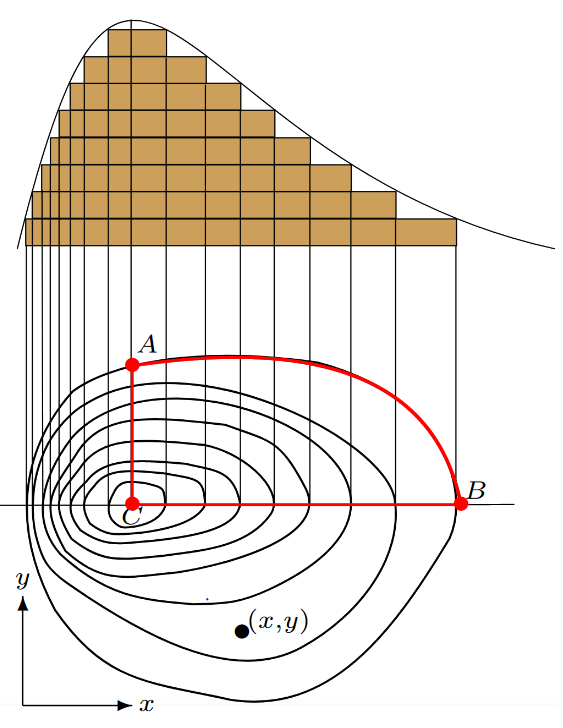
\includegraphics[scale=0.3]{./Bilder/Hoehenlinie.png}

\caption{\label{fig_Hoehen}%
Eine Karte mit H\"ohenlinien und die Frontalansicht
der zugeh\"origen Landschaft (aus \cite{Wiki_Hoehenlinie}). Eingetragen 
in rot ist ein Rundweg ($A\rightarrow B \rightarrow C \rightarrow A$) von der
Ebene auf die Spitze ($C$) des Berges. Jeder Punkt $(x,y)$ auf dieser Karte hat
eine wohl definierte H\"ohe -- die H\"ohe ist eine \glqq Zustandsgr\"o\ss e\grqq. Ob man \"uber
einen horizontalen Weg oder einen vertikalen Weg zu einem Punkt (z.B.\ $C$) gelangt ist, l\"asst sich dem
Punkt aber nicht ansehen.}
\end{SCfigure}

Wir betrachten ein zweidimensionales Gel\"ande, also eine Fl\"ache 
mit unterschiedlichen H\"ohen (siehe Abb.\ \ref{fig_Hoehen}).\index{Hoehenlinie@H\"ohenlinie}
Die H\"ohe $H$ eines Punktes $\pmb{x}=(x,y)$ ist eine \glqq Zustandsgr\"o\ss e\grqq, d.h.,
wenn der Punkt $\pmb{x}$ (z.B.\ sein L\"angen- und Breitengrad auf der Erde) bekannt
ist, k\"onnen wir die H\"ohe $H(\pmb{x})$ an diesem Punkt aus der Karte ablesen. 

Diese H\"ohe kann sich auf zwei Weisen (oder Linearkombinationen davon)
\"andern: Durch einen Schritt in Ost-West-Richtung ($x$-Achse) oder durch einen
Schritt in Nord-S\"ud-Richtung ($y$-Achse). In Analogie zu Gl.\ \ref{eq_ZuPro_Energie}
schreiben wir:
\begin{equation}
\label{eq_deltah}
         {\rm d}H = \delta X + \delta Y \, .
\end{equation}
Hierbei bezeichnet $\delta X$ eine H\"ohen\"anderung entlang der $x$-Richtung 
und $\delta Y$ eine H\"ohen\"anderung entlang der $y$-Richtung. Es gibt
keine Zustandsgr\"o\ss e zu $\delta X$ oder $\delta Y$ und man kann einem
Punkt $\pmb{x}$ auch nicht \glqq ansehen\grqq, ob man \"uber einen
Weg entlang der $x$-Achse oder entlang der $y$-Achse dorthin gelang ist. 
Trotzdem kann man jede H\"ohen\"anderung ${\rm d}H$ (diese erfolgt entlang eines
Weges) in einen Anteil entlang der $x$- und einen Anteil entlang der $y$-Achse zerlegen. 

Allgemein gilt f\"ur das totale Differential der H\"ohe:
\begin{equation}
    {\rm d}H = \frac{\partial H}{\partial x}{\rm d}x + \frac{\partial H}{\partial y} {\rm d} y \, . 
\end{equation}
Diese Gr\"o\ss e ist eine Prozessgr\"o\ss e. Man kann sie entlang eines Weges $\gamma: t \mapsto (x(t),y(t))$ 
integrieren und erh\"alt so:
\begin{equation}
             H(x,y) - H(x_0,y_0) = \int_\gamma {\rm d}H = \int_0^1 \left( \frac{\partial H}{\partial x}\frac{{\rm d}x}{{\rm d}t}
                     + \frac{\partial H}{\partial y} \frac{{\rm d} y}{{\rm d}t} \right) {\rm d}t \, ,
\end{equation}
wobei $(x_0,y_0)$ der Startpunkt des Weges und $(x,y)$ der Entdpunkt des Weges sein sollen. Man
beachte, dass
\begin{equation}
             \left( \frac{\partial H}{\partial x}\frac{{\rm d}x}{{\rm d}t}
         + \frac{\partial H}{\partial y} \frac{{\rm d} y}{{\rm d}t} \right) = \pmb{\nabla}H \cdot \frac{{\rm d} \pmb{x}}{{\rm d}t} \, .
\end{equation}


Die Gr\"o\ss en $x$ und $y$, also die Koordinaten eines Punktes, sind ebenfalls Zustandsgr\"o\ss en
f\"ur einen Punkt $\vec{x}=(x,y)$. Die Gr\"o\ss en
\begin{equation}
    \delta X = \frac{\partial H}{\partial x}{\rm d}x \hspace{1cm} {\rm und} \hspace{1cm}
    \delta Y = \frac{\partial H}{\partial y}{\rm d}y
\end{equation}
sind jedoch reine \glqq Prozessgr\"o\ss en\grqq, d.h., sie sind nur entlang bestimmter Wege
definiert (einmal entlang Wege in Ost-West-Richtung und einmal entlang Wege
in Nord-S\"ud-Richtung). Offenbar sind ${\rm d}x$ und ${\rm d}y$ die
Differentiale der Zustandsgr\"o\ss en zu den Koordinatenfunktionen $\pi_x(\vec{x})=x$ und
$\pi_y(\vec{x})=y$.
% und $\frac{\partial H}{\partial x}$ bzw.\ $\frac{\partial H}{\partial y}$ sind
%die zugeh\"origen \textit{integrierenden Faktoren}. 
Bei einer konsistenten Notation
sollte man daher besser ${\rm d}\pi_x$ statt ${\rm d}x$ und ${\rm d}\pi_y$ statt ${\rm d}y$ 
schreiben (siehe auch \cite{Straumann} zum Formalismus der Differentialformen in
der Thermodynamik).  

\section{Der Unterschied zwischen Arbeit und W\"arme}
\label{sec_ZuPro_Arbeit}

Meist wird in der Thermodynamik angenommen, dass die Aufteilung einer
\"Anderung der inneren Energie in einen Anteil \glqq Arbeit\grqq\ und einen Anteil \glqq W\"arme\grqq\
eindeutig vorgenommen werden kann.\index{Arbeit}\index{Waerme@W\"arme} 
Doch ein Blick auf die statistische Mechanik, die
der Thermodynamik zugrunde liegt, zeigt, dass diese Aufteilung nicht ganz so selbstverst\"andlich
ist. 

Die innere Energie $U$\index{Energie!innere}\index{Innere Energie} 
ist ein Erwartungswert: Es ist der Erwartungswert der Energie
f\"ur ein statistisches Ensemble. Ein statistisches Ensemble ist definiert durch die m\"oglichen
Mikrozust\"ande $i$, die es einnehmen kann, sowie durch eine Wahrscheinlichkeitsverteilung
$\{p_i\}$, mit der ein bestimmter Mikrozustand $i$ angenommen wird. Um welches Ensemble es sich
handelt und damit um welche Wahrscheinlichkeitsverteilung $\{p_i\}$ h\"angt davon ab, 
welche Parameter an einem System wir kontrollieren bzw.\ beobachten m\"ochten. 

Die beiden g\"angigen Ensembles in der Physik sind die mikrokanonische Gesamtheit und die 
kanonische Gesamtheit. In der\index{Gesamtheit!mikrokanonisch}\index{Mikrokanonische Gesamtheit} 
mikrokanonischen Gesamtheit kontrollieren wir die Gesamtenergie
des Systems (die W\"ande erlauben keinerlei Austausch von Energie mit der Umgebung), das
Volumen des Systems (die W\"ande sind starr), die Stoffmengen (die W\"ande lassen keinerlei
Form von Materie hindurch) sowie eventuell weitere Gr\"o\ss en. 
In diesem Fall ist die innere Energie $U$ gleich der Energie $E$, die jedem einzelnen Mikrozustand
zukommt und jeder m\"ogliche Mikrozustand hat dieselbe Wahrscheinlichkeit $p_i=1/|\Omega|$,
wobei $\Omega$ die Menge der m\"oglichen Mikrozust\"ande zu den vorgegebenen Bedingungen
(feste Energie, festes Volumen, feste Teilchenzahl, etc.) bezeichnet.

Die zweite g\"angige Gesamtheit ist die kanonische\index{Gesamtheit!kanonische}\index{Kanonische Gesamtheit} 
Gesamtheit, bei der das System 
einen \glqq thermischen\grqq\ Energieaustausch mit der Umgebung haben kann, jedoch sind
das Volumen und die Teilchenzahl bzw.\ die Stoffmengen fest. In diesem Fall ist die Wahrscheinlichkeitsverteilung
$\{p_i\}$ durch die Boltzmann-Verteilung gegeben: $p_i=\frac{1}{Z}\exp(-\beta E_i)$, d.h., die Wahrscheinlichkeit,
mit der ein bestimmter\index{Boltzmann-Verteilung} 
Mikrozustand mit der Energie $E_i$ in dem Ensemble vertreten ist, ist proportional 
zum Boltzmann-Faktor, wobei die Zustandssumme $Z=\sum_i \exp(-\beta E_i)$ die Wahrscheinlichkeiten
normiert. $\beta=1/k_{\rm B}T$ ist gleich dem Inversen der Boltzmann-Konstanten $k_{\rm B}$ und der
absoluten Temperatur $T$.

In jedem Ensemble ist die Energie $E_i$ eines erlaubten Zustands $i$ eine Funktion der
kontrollierten Parameter (Volumen $V$ oder Druck $p$, Gesamtenergie $E$ oder Temperatur $T$, 
Stoffmengen $n_i$ oder chemische Potenziale $\mu_i$, \"au\ss ere Felder, etc.), Alles, was nicht
kontrolliert wird, steckt in der Wahrscheinlichkeitsverteilung $\{p_i\}$, die somit ebenfalls von den
kontrollierten Parametern abh\"angt. Die innere Energie $U$ ist gegeben durch
\begin{equation}
                         U = \sum_i E_i p_i \, ,
\end{equation}
wobei die Summe \"uber alle zul\"assigen Mikrozust\"ande $i$ l\"auft und $E_i$ die Energie dieses
Mikrozustands ist. 

Eine \"Anderung von $U$ ist prinzipiell auf zwei Weisen m\"oglich:
\begin{equation}
                        {\rm d} U = \sum_i {\rm d}E_i \, p_i  + \sum_i E_i\,{\rm d}p_i  = - \delta W + \delta Q \, .
\end{equation}
Der erste Term, den wir als Arbeit interpretieren, beruht auf einer \"Anderung der Energie $E_i$ der
Mikrozust\"ande, weil die kontrollierten Parameter ge\"andert wurden. Der zweite Term, 
den wir als W\"arme interpretieren, beruht auf einer \"Anderung der Wahrscheinlichkeitsverteilung
$\{p_i\}$, die m\"oglicherweise mit einer \"Anderung dieser Parameter einhergeht.
Die Aufteilung einer \"Anderung der inneren Energie in Arbeit und W\"arme h\"angt somit 
entscheidend davon ab, welche Parameter wir beobachten bzw.\ kontrollieren. Straumann
schreibt dazu: \glqq Darum ist die W\"arme, und damit die Entropie [...], in der statistischen 
Mechanik streng genommen immer nur \underline{relativ} zu einem makroskopischen Beobachter
definiert.\grqq\ (\cite{Straumann}, Fu\ss note S.\ 21).

In der Thermodynamik k\"onnen wir den Begriff der Arbeit nur definieren, wenn wir wissen,
was \glqq adiabatische W\"ande\grqq\ sind, d.h, was \glqq thermisch abgeschlossen\grqq\
bedeutet. Ein adiabatischer Kolben repr\"asentiert eine Wand, bei der das Volumen eines
Systems sich \"andern kann (es kann beispielsweise an ein Druckbad angekoppelt werden), 
aber trotzdem wird keine W\"arme ausgetauscht. Ist die geleistete Arbeit $W$ entlang eines Weges
bekannt und ist bekannt, wie sich die Gesamtenergie $U$ bei diesem Prozess ge\"andert hat ($\Delta U$),
so definiert man die bei diesem Prozess geflossene W\"arme als $Q=\Delta U-W$. 

\section{1-Formen und \glqq infinitesimale Inkremente\grqq}

In der Physik interpretiert man die Differentiale in Gl.\ \ref{eq_ZuPro_Differential} oder in
Gl.\ \ref{eq_ZuPro_EinsForm} gerne als \glqq sehr kleine\grqq\ (infinitesimale) Differenzen
oder Inkremente. In diesem Abschnitt soll beschrieben werden, inwiefern diese Vorstellung
mit den bisherigen \"Uberlegungen zu 1-Formen als lineare Abbildungen vertr\"aglich
ist. 

Wir betrachten einen Punkt $p$ auf der Mannigfaltigkeit der Gleichgewichtszust\"ande, beschrieben
durch seine Koordinaten $\pmb{x}(p)=(x_1(p),...,x_n(p))$, sowie einen Tangentialvektor $\pmb{v}$ 
(eine \glqq Geschwindigkeit\grqq) an diesem Punkt (ausgedr\"uckt durch die lokalen Koordinaten). 
Zu diesen beiden Gr\"o\ss en betrachten wir einen Weg $\pmb{x}(t)$
auf der Mannigfaltigkeit, der in den lokalen Koordinaten um den Punkt $p$ durch
$\pmb{x}(t) = \pmb{x}(p) + \pmb{v} t$ gegeben ist, wobei $t\in[0,\Delta t]$. Das bedeutet, dieser
Weg ist nur sehr kurz und f\"uhrt von $p$ zu einem Nachbarpunkt $p'$, der die Koordinaten
$\pmb{x}(p')=\pmb{x}(p) +  \pmb{v} \Delta t$ hat. Wir bezeichnen mit $\Delta \pmb{x}(p) =
 \pmb{v} \Delta t $ ein (endliches) \glqq Inkrement\grqq\ in den Koordinaten. Dann gilt f\"ur
eine 1-Form $\omega_{(\pmb{x})}$, integriert entlang dieses Weges:
\begin{equation}
          \delta \Omega = \int_0^{\Delta t} \omega_{(\pmb{x}(t))}( \pmb{v})\, {\rm d}t \approx
            \omega_{(\pmb{x}(p))}( \pmb{v})\, \Delta t = \sum_{i=1}^n \omega_i(\pmb{x}) \Delta x_i
             \, .
\end{equation} 
F\"ur Prozesse, die durch sehr kurze Wege zwischen zwei eng benachbarten Gleichgewichtszust\"anden
beschrieben werden, ist die Darstellung durch \glqq kleine endliche Inkremente\grqq\ also durchaus
sinnvoll. Allerdings sollte man sich bewusst sein, dass im Allgemeinen $\delta \Omega$ keine  
\"Anderung oder Differenz einer in einer Umgebung von $p$ wohl definierten Funktion darstellt, 
sondern lediglich eine kleine Zahl ist, die einem Weg von dem Gleichgewichtszustand $p$ zu seinem 
benachbarten Gleichgewichtszustand $p'$ zugeordnet werden kann. Lediglich wenn $\omega_{(\pmb{x})}$
eine exakte 1-Form ist, kann man $\delta \Omega = \Delta \Omega$ als Differenz von 
einer Funktion $\Omega$ auffassen. 

  







\begin{thebibliography}{99}
\bibitem{Jauch} Jauch, Josef-Maria; \textit{Analytical Thermodynamics. Part I. Thermostatics --
        General Theory}; Foundations of Physics, Vol.\ 5, No.\ 1 (1975) 111--132.
\bibitem{Straumann} Straumann, Norbert; \textit{Thermodynamik}; Lecture Notes in Physics 265;
           Springer-Verlag 1986.        
\bibitem{Wiki_Hoehenlinie} Wikipedia \glqq H\"ohenlinie\grqq\ bzw.\ \glqq contour line\grqq. 
                        \url{https://en.wikipedia.org/wiki/Contour_line} (aufgerufen am 13.02.2024).           
\end{thebibliography}

\section*{Anmerkungen}
\subsection*{Vektorb\"undel}
\label{A_ZuPro_VB}

Ein Vektorb\"undel $(M,B,\pi,V)$ ist eine Mannigfaltigkeit $M$ sowie eine sogenannte Basismannigfaltigkeit
$B$ mit einer Projektion $ \pi: M \rightarrow B$, die jedem Punkt $p\in M$ eindeutig einen Punkt $\pi(p)\in B$
zuordnet, sodass das Urbild $\pi^{-1}(b)$ f\"ur jeden Punkt $b\in B$ isomorph ist zu dem Vektorraum $V$, also
$\pi^{-1}(b) \simeq V,~\forall b\in B$. Lokal, in einer offenen Umgebung $U$ eines Punktes $b$ der Basismannigfaltigkeit,
ist ein Vektorb\"undel isomorph zu $U \times V$.


\end{document}

